\section{Bit-Exact Reproduction and the Faithful Baseline}\label{sec:repro}

Every comparison in this study is anchored to implementations that are first
verified to be exact copies of their published references. This section
documents the verification gate, the faithful small-budget baseline trained on
the verified backbone, and where that baseline sits relative to the original
released model. It makes no comparative claims beyond that descriptive
placement.

\subsection{The verification gate}

The gate is a deterministic forward-logits comparison: the official
HuggingFace weights are loaded into our from-scratch \texttt{model.py}, a
single fixed prompt (``The capital of France is'', input shape $[1,5]$) is run
in fp32, and the next-token logits are compared element-wise against the
reference implementation, with a pass threshold of
$\max|\Delta\text{logits}| < 10^{-3}$ plus argmax agreement. For our
Qwen3-0.6B reproduction~\citep{yang2025qwen3} the recorded result is not
merely within tolerance but exact: $\max|\Delta\text{logits}| = 0.0$, relative
error $0.0$, and both implementations predict token id 12095 (`` Paris'')
(Table~\ref{tab:repro}). We state the protocol's scope plainly: it is one
prompt, fp32, forward logits only -- it establishes operator-level
implementation identity under the loaded weights, not behavioral equivalence
over an input distribution. The parameter count of 596{,}049{,}920 is the
forward-calculation total of the build's architecture plan, asserted (within
1\%) by the build's unit test, rather than a field written by the verification
artifact itself.

% tab_repro.tex -- reproduction verification gate
% Sources (re-read 2026-07-06):
%   Qwen3-0.6B/builds/2026-06-08_reproduce-faithful_qwen3-0.6b/results/verify.json
%   Qwen3-0.6B/builds/2026-06-08_reproduce-faithful_qwen3-0.6b/architecture_plan.md (param total, line 60)
%   SmolLM2-134(base)/results/param_count.log, parity.log, comparison_with_hf.md
\begin{table}[t]
\centering
\small
\setlength{\tabcolsep}{4.5pt}
\begin{tabular}{@{}llrlll@{}}
\toprule
Model & HF reference & Params & $\max|\Delta\text{logits}|$ & Argmax & Device \\
\midrule
Qwen3-0.6B (ours) & \texttt{Qwen/Qwen3-0.6B-Base} & 596{,}049{,}920 & $0.0$ & match & CPU/GPU fp32 \\
SmolLM2-135M (ours) & \texttt{HuggingFaceTB/SmolLM2-135M} & 134{,}515{,}008 & $0.0$ & match & CPU fp32 \\
\quad (same weights, GPU) & & & $4.72\times10^{-5}$ & match & GPU fp32 \\
\bottomrule
\end{tabular}
\caption{Reproduction verification against the HuggingFace reference weights.
Each check is a deterministic single-prompt fp32 forward-logits comparison
(tolerance $10^{-3}$; no training compute is compared, so no compute budget,
seeds, or variance estimate applies, and no eval-suite stamp applies).
Qwen3-0.6B: prompt ``The capital of France is'', identical next token
(id 12095, `` Paris''), \texttt{max\_abs\_error} and \texttt{relative\_error}
both exactly $0.0$ (\texttt{verify.json}); the parameter count is the
forward-calculation total asserted by the build's unit test
(\texttt{architecture\_plan.md}). SmolLM2-135M: bit-exact on CPU fp32
($\max|\Delta| = 0.0$, identical next token `` the'',
\texttt{parity.log}/\texttt{param\_count.log}); the same weights on GPU show
$\max|\Delta| = 4.72\times10^{-5}$, attributed to SDPA kernel-dispatch
reduction-order noise, not a weight or architecture difference
(\texttt{comparison\_with\_hf.md}).}
\label{tab:repro}
\end{table}


A second reproduction, SmolLM2-135M~\citep{allal2025smollm2} at
134{,}515{,}008 parameters, passes the same gate on CPU fp32 with
$\max|\Delta\text{logits}| = 0.0$ across the final logits and all 30 per-layer
hidden states, identical greedy generation on 5 of 5 probe prompts, and a
wikitext-2 validation perplexity of 15.371 identical to the HuggingFace
reference (Table~\ref{tab:repro}). The same weights evaluated on GPU show
$\max|\Delta\text{logits}| = 4.72\times10^{-5}$ (and $1.95\times10^{-3}$ in
the layer-14 hidden state), attributed to SDPA kernel-dispatch
reduction-order differences rather than any weight or architecture
discrepancy. This is a useful calibration: logit deltas at the
$10^{-5}$ scale on GPU are device noise, so ``bit-exact'' is a claim we make
only where the measured error is exactly zero.

\subsection{The faithful baseline at 1.19B tokens}

The faithful baseline trains the verified Qwen3-0.6B backbone from random
initialization for 18{,}150 steps at 65{,}536 tokens per step --
1{,}189{,}478{,}400 FineWeb-Edu tokens~\citep{penedo2024fineweb}, roughly two
tokens per parameter, four orders of magnitude below both the original 36T-token
budget and compute-optimal prescriptions~\citep{hoffmann2022training}. The
recipe is AdamW~\citep{loshchilov2017decoupled} with cosine decay from a peak
learning rate of $2.4\times10^{-3}$, bf16, sequence length 4096, seed 0;
Table~\ref{tab:hparams} flags each hyperparameter as reported or chosen by us.
In-loop validation perplexity descends from 185{,}810.49 at random
initialization -- close to the 151{,}936-way uniform-guessing level expected
of an untrained model -- through 60.10 at 2{,}000 steps to a final 28.65
(Figure~\ref{fig:ppl-curves}). All values on this curve are in-loop validation
perplexity from a single run, not suite-stamped.

\begin{figure}[t]
\centering
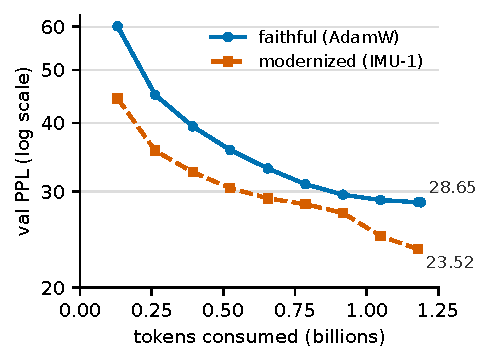
\includegraphics[width=0.72\linewidth]{figures/fig_ppl_curves.pdf}
\caption{In-loop validation perplexity versus consumed tokens for the faithful
baseline and the modernized IMU-1 build~\citep{grigorev2026imu} at the
identical 1{,}189{,}478{,}400-token budget (18{,}150 steps $\times$ 65{,}536
tok/step, FineWeb-Edu, seed 0). Single run per arm, trainer-internal
FineWeb-Edu validation eval, no suite stamp; endpoints are tabulated with
their independent suite-stamped scores in Table~\ref{tab:arms}, and no
comparative claim is drawn from these $n{=}1$ curves here. The faithful curve
ends at the post-training eval (28.65); the run completed in 2{,}663.1
minutes at 52.4\,GB peak memory. Sources:
\texttt{qwen3\_baseline2tpp\_train.log},
\texttt{qwen3\_imu1\_2tpp\_train.log}.}
\label{fig:ppl-curves}
\end{figure}

\subsection{Gap to the original}

The released \texttt{Qwen3-0.6B-Base}, trained on $\approx$36T tokens, scores
13.400 on the identical 300k-token FineWeb-Edu validation slice with identical
evaluation code (204{,}800 tokens scored, 50 windows $\times$ 4096). Our
1.19B-token baseline at 28.65 therefore sits at $2.14\times$ the original's
perplexity with $\approx$30{,}000$\times$ less data
(Figure~\ref{fig:repro-gap}). The earlier matched-compute learning-rate sweep
at $\approx$131M tokens per arm provides a second, smaller-budget point: its
best arm (peak LR $2.4\times10^{-3}$, carried forward to the full run) reached
46.310, a $3.5\times$ gap at $\approx$275{,}000$\times$ less data, with the
$1.7\times10^{-3}$ and $3.0\times10^{-3}$ arms at 46.892 and 49.276. The two
ratios belong to two different budgets and are never conflated. Both are
descriptive only -- single runs, in-loop trainer evals, no variance estimate
-- and locate the small-budget models on the same axis as the reference; they
are not parity claims.

\begin{figure}[t]
\centering
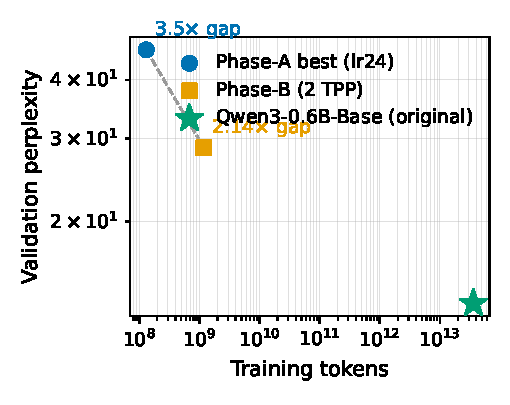
\includegraphics[width=0.72\linewidth]{figures/fig_repro_gap.pdf}
\caption{Gap to the original: validation perplexity versus training tokens on
the identical 300k-token FineWeb-Edu validation slice (204{,}800 tokens
scored, identical eval code). Original \texttt{Qwen3-0.6B-Base} 13.400 at
$\approx$36T tokens; faithful baseline 28.65 at 1{,}189{,}478{,}400 tokens
($2.14\times$ gap, $\approx$30{,}000$\times$ less data); best Phase~A
learning-rate-sweep arm 46.310 at $\approx$131M tokens ($3.5\times$ gap,
$\approx$275{,}000$\times$ less data). Single run per point, in-loop trainer
eval, not suite-stamped; descriptive only. Sources:
\texttt{original\_vs\_repro.txt}, \texttt{qwen3\_baseline2tpp\_after.txt}.}
\label{fig:repro-gap}
\end{figure}

\subsection{Suite-stamped scores for the baseline checkpoint}

Because the in-loop 28.65 lives on the trainer's own FineWeb-Edu validation
split, it is never compared against numbers from other corpora. The
independent evaluation harness stamps the same checkpoint at wikitext-2
perplexity 37.01 and code\_py perplexity 438.67 (text-lm-v2, 204{,}600 tokens
per corpus), each with a subsample noise floor -- 1.30 absolute
($\approx$3.7\%) on wikitext-2 but 280.56 absolute ($\approx$68.2\%) on
code\_py, so code-perplexity differences for this checkpoint are read as
directional only (Table~\ref{tab:arms}). These stamped values, not the
in-loop curve, are the baseline reference points for every cross-run
comparison in the following sections.
